\documentclass[11pt,oneside]{article}
\usepackage[T1]{fontenc}
\usepackage[utf8]{inputenc}
%\usepackage[latin1]{inputenc}
\DeclareUnicodeCharacter{00A0}{ }
% \usepackage{lmodern}
%\usepackage[adobe-utopia,uppercase=upright,greeklowercase=upright]{mathdesign}
\usepackage[adobe-utopia]{mathdesign}
%\usepackage{minionpro}
% \usepackage{pifont}
% \usepackage{amssymb}
\usepackage{amsmath}
\usepackage[francais]{babel}
% \usepackage[francais]{varioref}
\usepackage[dvips]{graphicx}
\usepackage{here}
\usepackage{framed}
\usepackage[normalem]{ulem}
\usepackage{fancyhdr}
\usepackage{titlesec}
\usepackage{vmargin}
\usepackage{longtable}

\usepackage{amsmath}

\usepackage{ifthen}
%\usepackage[•]{caption}

%\usepackage{epsfig}
\usepackage{subfig}

\usepackage{multirow}
\usepackage{multicol} % Portions de texte en colonnes
\usepackage{flafter}%floatants après la référence



\usepackage{color}
\usepackage{colortbl}


\definecolor{gris25}{gray}{0.75}
\definecolor{bleu}{RGB}{18,33,98}
\definecolor{bleuf}{RGB}{42,94,171}
\definecolor{bleuc}{RGB}{231,239,247}
\definecolor{rougef}{RGB}{185,18,27}
\definecolor{rougec}{RGB}{255,230,231}
\definecolor{vertf}{RGB}{103,126,82}
\definecolor{vertc}{RGB}{220,255,191}
\definecolor{violetf}{RGB}{112,48,160}
\definecolor{violetc}{RGB}{230,224,236}
\definecolor{jaunec}{RGB}{220,255,191}


\newenvironment{corrige}[1][\hsize]%
{%
    \def\FrameCommand
    {%
\rotatebox{90}{\textit{\textsf{Correction}}} 
        {\color{violetf}\vrule width 3pt}%
        \hspace{0pt}%must no space.
        \fboxsep=\FrameSep\colorbox{violetc}%
    }%
    \MakeFramed{\hsize#1\advance\hsize-\width\FrameRestore}%
}%
{\endMakeFramed}%



\newenvironment{sci}[1][\hsize]%
{%
    \def\FrameCommand%
    {%
%\rotatebox{90}{\textit{\textsf{Scilab}}
\includegraphics[height=.8cm]{png/logo_scilab}} 
\rotatebox{90}{
\includegraphics[height=.6cm]{png/logo_scilab}} 
        {\color{violetf}\vrule width 3pt}%
        \hspace{0pt}%must no space.
        \fboxsep=\FrameSep\colorbox{violetc}%
    }%
    \MakeFramed{\hsize #1 \advance\hsize-\width\FrameRestore}%
}%
{\endMakeFramed}%

\newenvironment{pseudo}[1][\hsize]%
{%
    \def\FrameCommand%
    {%
\rotatebox{90}{\textit{\textsf{Pseudo Code}}} 
        {\color{violetf}\vrule width 3pt}%
        \hspace{0pt}%must no space.
        \fboxsep=\FrameSep\colorbox{violetc}%
    }%
    \MakeFramed{\hsize #1 \advance\hsize-\width\FrameRestore}%
}%
{\endMakeFramed}%

\newenvironment{py}[1][\hsize]%
{%prof
    \def\FrameCommand%
    {%
%\rotatebox{90}{\textit{\textsf{Python}}} 
\rotatebox{90}{
\includegraphics[height=.6cm]{png/logo_python}} 
        {\color{violetf}\vrule width 3pt}%
        \hspace{0pt}%must no space.
        \fboxsep=\FrameSep\colorbox{violetc}%
    }%
    \MakeFramed{\hsize #1 \advance\hsize-\width\FrameRestore}%
}%
{\endMakeFramed}%


\newenvironment{term}[1][\hsize]%
{%
    \def\FrameCommand%
    {%
\rotatebox{90}{\textit{\textsf{Terminal}}} 
        {\color{violetf}\vrule width 3pt}%
        \hspace{0pt}%must no space.
        \fboxsep=\FrameSep\colorbox{violetc}%
    }%
    \MakeFramed{\hsize #1 \advance\hsize-\width\FrameRestore}%
}%
{\endMakeFramed}%


\newenvironment{rem}[1][\hsize]%
{%
    \def\FrameCommand
    {%
\rotatebox{90}{\textit{\textsf{Remarque}}} 
        {\color{bleuf}\vrule width 3pt}%
        \hspace{0pt}%must no space.
        \fboxsep=\FrameSep\colorbox{bleuc}%
    }%
    \MakeFramed{\hsize#1\advance\hsize-\width\FrameRestore}%
}%
{\endMakeFramed}%


\newenvironment{savoir}[1][\hsize]%
{%
    \def\FrameCommand
    {%
\rotatebox{90}{\textit{\textsf{Savoir}}} 
        {\color{bleuf}\vrule width 3pt}%
        \hspace{0pt}%must no space.
        \fboxsep=\FrameSep\colorbox{bleuc}%
    }%
    \MakeFramed{\hsize#1\advance\hsize-\width\FrameRestore}%
}%
{\endMakeFramed}%

\newenvironment{Objectif}[1][\hsize]%
{%
    \def\FrameCommand
    {%
\rotatebox{90}{\textit{\textsf{Objectif}}} 
        {\color{bleuf}\vrule width 3pt}%
        \hspace{0pt}%must no space.
        \fboxsep=\FrameSep\colorbox{bleuc}%
    }%
    \MakeFramed{\hsize#1\advance\hsize-\width\FrameRestore}%
}%
{\endMakeFramed}%

\newenvironment{prob}[1][\hsize]%prof
{%
    \def\FrameCommand%
    {%
\rotatebox{90}{\textit{\textsf{ Problématique}}} 
        {\color{rougef}\vrule width 3pt}%
        \hspace{0pt}%must no space.
        \fboxsep=\FrameSep\colorbox{rougec}%
    }%
    \MakeFramed{\hsize#1\advance\hsize-\width\FrameRestore}%
}%
{\endMakeFramed}%

\newenvironment{obj}[1][\hsize]%
{%
    \def\FrameCommand%
    {%
\rotatebox{90}{\textit{\textsf{ $\;$}}} 
        {\color{rougef}\vrule width 3pt}%
        \hspace{0pt}%must no space.
        \fboxsep=\FrameSep\colorbox{rougec}%
    }%
    \MakeFramed{\hsize#1\advance\hsize-\width\FrameRestore}%
}%
{\endMakeFramed}%

\newenvironment{defi}[1][\hsize]%
{%
    \def\FrameCommand%
    {%
\rotatebox{90}{\textit{\textsf{Définition\\}}} 
        {\color{bleuf}\vrule width 3pt}%
        \hspace{0pt}%must no space.
        \fboxsep=\FrameSep\colorbox{bleuc}%
    }%
    \MakeFramed{\hsize#1\advance\hsize-\width\FrameRestore}%
}%
{\endMakeFramed}%


\newenvironment{demo}[1][\hsize]%
{%
    \def\FrameCommand%
    {%
\rotatebox{90}{\textit{\textsf{Démonstration\\}}} 
        {\color{bleuf}\vrule width 3pt}%
        \hspace{0pt}%must no space.
        \fboxsep=\FrameSep\colorbox{bleuc}%
    }%
    \MakeFramed{\hsize#1\advance\hsize-\width\FrameRestore}%
}%
{\endMakeFramed}%


\newenvironment{hypo}[1][\hsize]%
{%
    \def\FrameCommand%
    {%
\rotatebox{90}{\textit{\textsf{Hypothèse\\}}} 
        {\color{bleuf}\vrule width 3pt}%
        \hspace{0pt}%must no space.
        \fboxsep=\FrameSep\colorbox{bleuc}%
    }%
    \MakeFramed{\hsize#1\advance\hsize-\width\FrameRestore}%
}%
{\endMakeFramed}%


\newenvironment{prop}[1][\hsize]%
{%
    \def\FrameCommand%
    {%
\rotatebox{90}{\textit{\textsf{Propriété\\}}} 
        {\color{bleuf}\vrule width 3pt}%
        \hspace{0pt}%must no space.
        \fboxsep=\FrameSep\colorbox{bleuc}%
    }%
    \MakeFramed{\hsize#1\advance\hsize-\width\FrameRestore}%
}%
{\endMakeFramed}%

\newenvironment{props}[1][\hsize]%
{%
    \def\FrameCommand%
    {%
\rotatebox{90}{\textit{\textsf{Propriétés\\}}} 
        {\color{bleuf}\vrule width 3pt}%
        \hspace{0pt}%must no space.
        \fboxsep=\FrameSep\colorbox{bleuc}%
    }%
    \MakeFramed{\hsize#1\advance\hsize-\width\FrameRestore}%
}%
{\endMakeFramed}%

\newenvironment{exemple}[1][\hsize]%
{%
    \def\FrameCommand%
    {%
\rotatebox{90}{\textit{\textsf{Exemple\\}}} 
        {\color{vertf}\vrule width 3pt}%
        \hspace{0pt}%must no space.
        \fboxsep=\FrameSep\colorbox{vertc}%
    }%
    \MakeFramed{\hsize#1\advance\hsize-\width\FrameRestore}%
}%
{\endMakeFramed}%

\newenvironment{exercice}[1][\hsize]%
{%
    \def\FrameCommand%
    {%
\rotatebox{90}{\textit{\textsf{Exercice\\}}} 
        {\color{vertf}\vrule width 3pt}%
        \hspace{0pt}%must no space.
        \fboxsep=\FrameSep\colorbox{vertc}%
    }%
    \MakeFramed{\hsize#1\advance\hsize-\width\FrameRestore}%
}%
{\endMakeFramed}%

\newenvironment{Support}[1][\hsize]%
{%
    \def\FrameCommand%
    {%
\rotatebox{90}{\textit{\textsf{Support de cours\\}}} 
        {\color{vertf}\vrule width 3pt}%
        \hspace{0pt}%must no space.
        \fboxsep=\FrameSep\colorbox{jaunec}%
    }%
    \MakeFramed{\hsize#1\advance\hsize-\width\FrameRestore}%
}%
{\endMakeFramed}%

\newenvironment{resultat}[1][\hsize]%
{%
    \def\FrameCommand%
    {%
\rotatebox{90}{\textit{\textsf{Résultat\\}}} 
        {\color{rougef}\vrule width 3pt}%
        \hspace{0pt}%must no space.
        \fboxsep=\FrameSep\colorbox{rougec}%
    }%
    \MakeFramed{\hsize#1\advance\hsize-\width\FrameRestore}%
}%
{\endMakeFramed}%

\newenvironment{methode}[1][\hsize]%
{%
    \def\FrameCommand%
    {%
\rotatebox{90}{\textit{\textsf{Méthode\\}}} 
        {\color{rougef}\vrule width 3pt}%
        \hspace{0pt}%must no space.
        \fboxsep=\FrameSep\colorbox{rougec}%
    }%
    \MakeFramed{\hsize#1\advance\hsize-\width\FrameRestore}%
}%
{\endMakeFramed}%

\newenvironment{theo}[1][\hsize]%
{%
    \def\FrameCommand%
    {%
\rotatebox{90}{\textit{\textsf{Théorème\\}}} 
        {\color{rougef}\vrule width 3pt}%
        \hspace{0pt}%must no space.
        \fboxsep=\FrameSep\colorbox{rougec}%
    }%
    \MakeFramed{\hsize#1\advance\hsize-\width\FrameRestore}%
}%
{\endMakeFramed}%

\newenvironment{warn}[1][\hsize]%
{%
    \def\FrameCommand%
    {%
\rotatebox{90}{\textit{\textsf{Attention\\}}} 
        {\color{rougef}\vrule width 3pt}%
        \hspace{0pt}%must no space.
        \fboxsep=\FrameSep\colorbox{rougec}%
    }%
    \MakeFramed{\hsize#1\advance\hsize-\width\FrameRestore}%
}%
{\endMakeFramed}%

% \usepackage{pstricks}
%\usepackage{minitoc}
% \setcounter{minitocdepth}{4}

\setcounter{tocdepth}{2}

% \mtcselectlanguage{french} 

%\usepackage{draftcopy}% "Brouillon"
% \usepackage{floatflt}
\usepackage{psfrag}
%\usepackage{listings} % Permet d'insérer du code de programmation
\renewcommand{\baselinestretch}{1.2}

% Changer la numérotation des figures :
% ------------------------------------
% \makeatletter
% \renewcommand{\thefigure}{\ifnum \c@section>\z@ \thesection.\fi
%  \@arabic\c@figure}
% \@addtoreset{figure}{section}
% \makeatother
 


%%%%%%%%%%%%
% Définition des vecteurs %
%%%%%%%%%%%%
 \newcommand{\vect}[1]{\overrightarrow{#1}}

%%%%%%%%%%%%
% Définition des torseusr %
%%%%%%%%%%%%

 \newcommand{\torseur}[1]{%
\left\{{#1}\right\}
}

\newcommand{\torseurcin}[3]{%
\left\{\mathcal{#1} \left(#2/#3 \right) \right\}
}

\newcommand{\torseurstat}[3]{%
\left\{\mathcal{#1} \left(#2\rightarrow #3 \right) \right\}
}

 \newcommand{\torseurc}[8]{%
%\left\{#1 \right\}=
\left\{
{#1}
\right\}
 = 
\left\{%
\begin{array}{cc}%
{#2} & {#5}\\%
{#3} & {#6}\\%
{#4} & {#7}\\%
\end{array}%
\right\}_{#8}%
}

 \newcommand{\torseurcol}[7]{
\left\{%
\begin{array}{cc}%
{#1} & {#4}\\%
{#2} & {#5}\\%
{#3} & {#6}\\%
\end{array}%
\right\}_{#7}%
}

 \newcommand{\torseurl}[3]{%
%\left\{\mathcal{#1}\right\}_{#2}=%
\left\{%
\begin{array}{l}%
{#1} \\%
{#2} %
\end{array}%
\right\}_{#3}%
}

 \newcommand{\vectv}[3]{%
\vect{V\left( {#1} \in {#2}/{#3}\right)}
}


\newcommand{\vectf}[2]{%
\vect{R\left( {#1} \rightarrow {#2}\right)}
}

\newcommand{\vectm}[3]{%
\vect{\mathcal{M}\left( {#1}, {#2} \rightarrow {#3}\right)}
}


 \newcommand{\vectg}[3]{%
\vect{\Gamma \left( {#1} \in {#2}/{#3}\right)}
}

 \newcommand{\vecto}[2]{%
\vect{\Omega\left( {#1}/{#2}\right)}
}
% }$$\left\{\mathcal{#1} \right\}_{#2} =%
% \left\{%
% \begin{array}{c}%
%  #3 \\%
%  #4 %
% \end{array}%
% \right\}_{#5}}

%  ------------------------------------------
% | Modification du formatage des sections : | 
%  ------------------------------------------

% Grands titres :
% ---------------

\newcommand{\titre}[1]{%
\begin{center}
      \bigskip
      \rule{\textwidth}{1pt}
      \par\vspace{0.1cm}
      
      \textbf{\large #1}
      \par\rule{\textwidth}{1pt}
    \end{center}
    \bigskip
  }

% Supprime le numéro du chapitre dans la numérotation des sections:
% -----------------------------------------------------------------
\makeatletter
\renewcommand{\thesection}{\@arabic\c@section}
\makeatother


% \titleformat{\chapter}[display]
% {\normalfont\Large\filcenter}
% {}
% {1pc}
% {\titlerule[1pt]
%   \vspace{1pc}%
%   \Huge}[\vspace{1ex}%
% \titlerule]


%%%% Chapitres Comme PY Pechard %%%%%%%%%
% numéro du chapitre
\DeclareFixedFont{\chapnumfont}{OT1}{phv}{b}{n}{80pt}
% pour le mot « Chapitre »
\DeclareFixedFont{\chapchapfont}{OT1}{phv}{m}{it}{40pt}
% pour le titre
\DeclareFixedFont{\chaptitfont}{T1}{phv}{b}{n}{25pt}

\definecolor{gris}{gray}{0.75}
\titleformat{\chapter}[display]%
	{\sffamily}%
	{\filleft\chapchapfont\color{gris}\chaptertitlename\
	\\
	\vspace{12pt}
	\chapnumfont\thechapter}%
	{16pt}%
	{\filleft\chaptitfont}%
	[\vspace{6pt}\titlerule\titlerule\titlerule]

%%%%  Fin Chapitres Comme PY Pechard %%%%%%%%%


% Section, subsection, subsubsection sans serifs :
% % ----------------------------------------------

% \makeatletter
% \renewcommand{\section}{\@startsection{section}{0}{0mm}%
% {\baselineskip}{.3\baselineskip}%
% {\normalfont\sffamily\Large\textbf}}%
% \makeatother

\makeatletter
\renewcommand{\@seccntformat}[1]{{\textcolor{bleu}{\csname
the#1\endcsname}\hspace{0.5em}}}
\makeatother

\makeatletter
\renewcommand{\section}{\@startsection{section}{1}{\z@}%
                       {-4ex \@plus -1ex \@minus -.4ex}%
                       {1ex \@plus.2ex }%
                       {\normalfont\Large\sffamily\bfseries}}%
\makeatother
 
\makeatletter
\renewcommand{\subsection}{\@startsection {subsection}{2}{\z@}
                          {-3ex \@plus -0.1ex \@minus -.4ex}%
                          {0.5ex \@plus.2ex }%
                          {\normalfont\large\sffamily\bfseries}}
\makeatother
 
\makeatletter
\renewcommand{\subsubsection}{\@startsection {subsubsection}{3}{\z@}
                          {-2ex \@plus -0.1ex \@minus -.2ex}%
                          {0.2ex \@plus.2ex }%
                          {\normalfont\large\sffamily\bfseries}}
\makeatother
 
\makeatletter             
\renewcommand{\paragraph}{\@startsection{paragraph}{4}{\z@}%
                                    {-2ex \@plus-.2ex \@minus .2ex}%
                                    {0.1ex}%               
{\normalfont\sffamily\bfseries}}
\makeatother
 



\makeatletter             
\renewcommand{\subparagraph}{\@startsection{subparagraph}{5}{\z@}%
                                    {-2ex \@plus-.2ex \@minus .2ex}%
                                    {0.1ex}%               
{\normalfont\bfseries Question }}
\makeatother
\renewcommand{\thesubparagraph}{\arabic{subparagraph}} 
\makeatletter

\setcounter{secnumdepth}{5}


%  --------
% | Marges |
%  --------


% \setmarginsrb{2.5cm}{1.5cm}{2.5cm}{2cm}{1cm}{1cm}{1cm}{1cm}
\setmarginsrb{1.5cm}{1cm}{1cm}{1.5cm}{1cm}{1cm}{1cm}{1cm}

% Changer les marges localement :
% -----------------------------
\newenvironment{changemargin}[2]{\begin{list}{}{%
\setlength{\topsep}{0pt}%
\setlength{\leftmargin}{0pt}%
\setlength{\rightmargin}{0pt}%
\setlength{\listparindent}{\parindent}%
\setlength{\itemindent}{\parindent}%
\setlength{\parsep}{0pt plus 1pt}%
\addtolength{\leftmargin}{#1}%
\addtolength{\rightmargin}{#2}%
}\item }{\end{list}}



\usepackage{pst-solides3d}
\usepackage{titletoc}
\titlecontents{chapter}[+3pc]
  {\addvspace{10pt}\sffamily\bfseries}
{\contentslabel[{\pscirclebox[fillstyle=solid,fillcolor=gray!25,
linecolor=gray!25,framesep=4pt]{\textcolor{white}{\thecontentslabel}}}]{2.5pc}}
  {}
  {\dotfill \normalfont\thecontentspage\ }

\titlecontents{section}[3pc]
  {\addvspace{2pt}\sffamily}
  {\contentslabel[\thecontentslabel]{1.8pc}}
  {}
  {\dotfill \normalfont\thecontentspage\ }

\titlecontents{subsection}[5pc]
  {\addvspace{2pt}\sffamily}
  {\contentslabel[\thecontentslabel]{1.8pc}}
  {}
  {\dotfill \normalfont\thecontentspage\ }

\titlecontents{subsubsection}[8pc]
  {\addvspace{2pt}\sffamily}
  {\contentslabel[\thecontentslabel]{3pc}}
  {}
  {\dotfill \normalfont\thecontentspage\ }
%{\;\titlerule\;\normalfont\thecontentspage\ }

\titlecontents{paragraph}[9pc]
  {\addvspace{2pt}\sffamily}
  {\contentslabel[\thecontentslabel]{3.5pc}}
  {}
  {\dotfill \normalfont\thecontentspage\ }

%pour avoir l indentation dans minipage
\newdimen\oldparindent\oldparindent=\parindent

\makeatletter
\def\@iiiminipage#1#2[#3]#4{%
  \noindent
  \leavevmode
  \@pboxswfalse
  \setlength\@tempdima{#4}%
  \def\@mpargs{{#1}{#2}[#3]{#4}}%
  \setbox\@tempboxa\vbox\bgroup
    \color@begingroup
      \hsize\@tempdima
      \textwidth\hsize \columnwidth\hsize
      \@parboxrestore
      \parindent=\oldparindent
      \def\@mpfn{mpfootnote}\def\thempfn{\thempfootnote}\c@mpfootnote\z@
      \let\@footnotetext\@mpfootnotetext
      \let\@listdepth\@mplistdepth \@mplistdepth\z@
      \@minipagerestore
      \@setminipage}
\makeatother

%Definition de la commande question
\newcounter{Qu}
\newcommand{\Question}[2][0]{
\ifthenelse{\equal{#1}{0}}                      %demande-t-on une minipage ?
{\medskip\noindent {\refstepcounter{Qu}\textbf{Q\theQu .\hspace{0,7mm}}#2}\ifshowanswers \else \smallskip \fi}  %non donc on balance le texte
{\ifshowanswers                                 %oui minipage en mode problem
\noindent {\refstepcounter{Qu}\textbf{Q\theQu .\hspace{0,7mm}}#2}    %mode solution
\else                                           %mode problem
\noindent\begin{minipage}{#1}\noindent {\refstepcounter{Qu}\textbf{Q\theQu .\hspace{0,7mm}}#2}\end{minipage}\smallskip
\fi }
}

\newcommand{\Questionpb}[2][0]{%le premier argument entre [] est par défaut à 0
\begin{onlyproblem}\Question[#1]{#2}\end{onlyproblem}
}

\newcommand{\Onlyproblem}[2][0]{%le premier argument entre [] est par défaut à 0
%si le 2e arguement est 0
\ifthenelse{\equal{#1}{0}}
%on demande un environnement pb classique
{\begin{onlyproblem}#2\end{onlyproblem}}
%sinon on demande à faire une minipage
{\begin{onlyproblem}\noindent\begin{minipage}{#1}\parskip2ex #2\end{minipage}\smallskip \end{onlyproblem} }
}

\newcounter{Sl}
\addtocounter{Sl}{+1}
\newcommand{\Solutioncnt}[1]{\bigskip\noindent \textbf{R\theSl .\hspace{0,7mm}}\addtocounter{Sl}{+1} #1}
\newcommand{\Solutionnorm}[1]{#1}

\newif\ifmixte
\let\mixte\mixtetrue
\let\nomix\mixtefalse
\nomix

\newcommand{\Solution}[1]{
\noindent
\ifmixte
\noindent\rule[0.1cm]{17cm}{0.8pt}\\
  \begin{solution}
    \ifnum\theQu>0
    \Solutionnorm{#1}
    \else
    \Solutioncnt{#1}
    \fi
    \smallskip
  \end{solution}

\noindent\rule[0.1cm]{17cm}{0.8pt}
\else
  \begin{onlysolution}
\fbox{\parbox{\linewidth-2\fboxrule-2\fboxsep}{
    \ifnum\theQu>0
    \Solutionnorm{#1}
    \else
    \Solutioncnt{#1}
    \fi
    \smallskip
}}
  \end{onlysolution}
\fi
}

%\usepackage{algorithm}
%\usepackage{algorithmic}
\usepackage[french]{algorithm2e}

\SetKwBlock{Fonction}{Début Fonction}{Fin Fonction}
\SetKwComment{Comment}{start}{end}
% Python sources

\usepackage{listings}
\lstloadlanguages{R}   % pour regler les pb d accent utf8 dans les codes
\lstset{language=R} % pour regler les pb d accent utf8 dans les codes

\usepackage{textcomp}
\usepackage{setspace}
%\usepackage{palatino}

%\usepackage{color}
\definecolor{Bleu}{rgb}{0.1,0.1,1.0}
\definecolor{Noir}{rgb}{0,0,0}
\definecolor{Grau}{rgb}{0.5,0.5,0.5}
\definecolor{DunkelGrau}{rgb}{0.15,0.15,0.15}
\definecolor{Hellbraun}{rgb}{0.5,0.25,0.0}
\definecolor{Magenta}{rgb}{1.0,0.0,1.0}
\definecolor{Gris}{gray}{0.5}
\definecolor{Vert}{rgb}{0,0.5,0}
\definecolor{SourceHintergrund}{rgb}{1,1.0,0.95}


%
\renewcommand{\lstlistlistingname}{Listings}
\renewcommand{\lstlistingname}{Listing}

\lstnewenvironment{python}[1][]{
\lstset{
%escapeinside={\%*}{*)},
%inputencoding=utf8,   % pour regler les pb d accent utf8 dans les codes
%extendedchars=true,   % pour regler les pb d accent utf8 dans les codes
language=python,
basicstyle=\sffamily\footnotesize, 	
stringstyle=\color{red}, 
showstringspaces=false, 
alsoletter={1234567890},
otherkeywords={\ , \}, \{},
keywordstyle=\color{blue},
emph={access,and,break,class,continue,def,del,elif ,else,
except,exec,finally,for,from,global,if,import,in,i s,
lambda,not,or,pass,print,raise,return,try,while},
emphstyle=\color{black}\bfseries,
emph={[2]True, False, None, self},
emphstyle=[2]\color{olive},
emph={[3]from, import, as},
emphstyle=[3]\color{blue},
upquote=true,
columns=flexible, % pour empecher d'avoir un espacement mono
morecomment=[s]{"""}{"""},
commentstyle=\color{Hellbraun}\slshape, 
%emph={[4]1, 2, 3, 4, 5, 6, 7, 8, 9, 0},
emphstyle=[4]\color{blue},
literate=*{:}{{\textcolor{blue}:}}{1}
{=}{{\textcolor{blue}=}}{1}
{-}{{\textcolor{blue}-}}{1}
{+}{{\textcolor{blue}+}}{1}
{*}{{\textcolor{blue}*}}{1}
{!}{{\textcolor{blue}!}}{1}
{(}{{\textcolor{blue}(}}{1}
{)}{{\textcolor{blue})}}{1}
{[}{{\textcolor{blue}[}}{1}
{]}{{\textcolor{blue}]}}{1}
{<}{{\textcolor{blue}<}}{1}
{>}{{\textcolor{blue}>}}{1}
{COMPLETER}{{\textcolor{red}COMPLETER}}{1},
literate=%
            {é}{{\'{e}}}1
            {è}{{\`{e}}}1
            {ê}{{\^{e}}}1
            {ë}{{\¨{e}}}1
            {û}{{\^{u}}}1
            {ù}{{\`{u}}}1
            {â}{{\^{a}}}1
            {à}{{\`{a}}}1
            {î}{{\^{i}}}1
            {ç}{{\c{c}}}1
            {Ç}{{\c{C}}}1
            {É}{{\'{E}}}1
            {Ê}{{\^{E}}}1
            {À}{{\`{A}}}1
            {Â}{{\^{A}}}1
            {Î}{{\^{I}}}1, % pour regler les pb d accent utf8 dans les codes
%framexleftmargin=1mm, framextopmargin=1mm, frame=shadowbox, rulesepcolor=\color{blue},#1
%backgroundcolor=\color{SourceHintergrund}, 
%framexleftmargin=1mm, framexrightmargin=1mm, framextopmargin=1mm, frame=single, framerule=1pt, rulecolor=\color{black},#1
}}{}



\lstnewenvironment{scilab}[1][]{
\lstset{
language=scilab,
basicstyle=\sffamily\footnotesize, 	
stringstyle=\color{red}, 
showstringspaces=false, 
alsoletter={1234567890},
otherkeywords={\ , \}, \{},
keywordstyle=\color{blue},
emph={access,and,break,class,continue,def,del,elif ,else,
except,exec,finally,for,from,global,if,import,in,i s,
lambda,not,or,pass,print,raise,return,try,while,Debut},
emphstyle=\color{black}\bfseries,
emph={[2]True, False, None, self},
emphstyle=[2]\color{olive},
emph={[3]from, import, as},
emphstyle=[3]\color{blue},
upquote=true,
columns=flexible, % pour empecher d'avoir un espacement mono
morecomment=[s]{"""}{"""},
commentstyle=\color{Hellbraun}\slshape, 
%emph={[4]1, 2, 3, 4, 5, 6, 7, 8, 9, 0},
emphstyle=[4]\color{blue},
literate=*{:}{{\textcolor{blue}:}}{1}
{=}{{\textcolor{blue}=}}{1}
{-}{{\textcolor{blue}-}}{1}
{+}{{\textcolor{blue}+}}{1}
{*}{{\textcolor{blue}*}}{1}
{!}{{\textcolor{blue}!}}{1}
{(}{{\textcolor{blue}(}}{1}
{)}{{\textcolor{blue})}}{1}
{[}{{\textcolor{blue}[}}{1}
{]}{{\textcolor{blue}]}}{1}
{<}{{\textcolor{blue}<}}{1}
{>}{{\textcolor{blue}>}}{1},
%framexleftmargin=1mm, framextopmargin=1mm, frame=shadowbox, rulesepcolor=\color{blue},#1
%backgroundcolor=\color{SourceHintergrund}, 
%framexleftmargin=1mm, framexrightmargin=1mm, framextopmargin=1mm, frame=single, framerule=1pt, rulecolor=\color{black},#1
}}{}


\lstdefinestyle{stylepython}{%
escapeinside={\%*}{*)},
inputencoding=utf8,   % pour regler les pb d accent utf8 dans les codes
extendedchars=true,   % pour regler les pb d accent utf8 dans les codes
language=python,
basicstyle=\sffamily\footnotesize, 	
stringstyle=\color{red}, 
showstringspaces=false, 
alsoletter={1234567890},
otherkeywords={\ , \}, \{},
keywordstyle=\color{blue},
emph={access,and,break,class,continue,def,del,elif ,else,
except,exec,finally,for,from,global,if,import,in,i s,
lambda,not,or,pass,print,raise,return,try,while},
emphstyle=\color{black}\bfseries,
emph={[2]True, False, None, self},
emphstyle=[2]\color{green},
emph={[3]from, import, as},
emphstyle=[3]\color{blue},
upquote=true,
columns=flexible, % pour empecher d'avoir un espacement mono
morecomment=[s]{"""}{"""},
commentstyle=\color{Hellbraun}\slshape, 
%emph={[4]1, 2, 3, 4, 5, 6, 7, 8, 9, 0},
emphstyle=[4]\color{blue},
literate=*{:}{{\textcolor{blue}:}}{1}
{=}{{\textcolor{blue}=}}{1}
{-}{{\textcolor{blue}-}}{1}
{+}{{\textcolor{blue}+}}{1}
{*}{{\textcolor{blue}*}}{1}
{!}{{\textcolor{blue}!}}{1}
{(}{{\textcolor{blue}(}}{1}
{)}{{\textcolor{blue})}}{1}
{[}{{\textcolor{blue}[}}{1}
{]}{{\textcolor{blue}]}}{1}
{<}{{\textcolor{blue}<}}{1}
{>}{{\textcolor{blue}>}}{1}
{COMPLETER}{{\textcolor{red}COMPLETER}}{1},
literate=%
            {é}{{\'{e}}}1
            {è}{{\`{e}}}1
            {ê}{{\^{e}}}1
            {ë}{{\¨{e}}}1
            {û}{{\^{u}}}1
            {ù}{{\`{u}}}1
            {â}{{\^{a}}}1
            {à}{{\`{a}}}1
            {î}{{\^{i}}}1
            {ç}{{\c{c}}}1
            {Ç}{{\c{C}}}1
            {É}{{\'{E}}}1
            {Ê}{{\^{E}}}1
            {À}{{\`{A}}}1
            {Â}{{\^{A}}}1
            {Î}{{\^{I}}}1,
%numbers=left,                    % where to put the line-numbers; possible values are (none, left, right)
%numbersep=5pt,                   % how far the line-numbers are from the code
%numberstyle=\tiny\color{mygray}, % the style that is used for the line-numbers
}

%
%\renewcommand{\algorithmicrequire} {\textbf{\textsc{Entrées:}}}
%\renewcommand{\algorithmicensure}  {\textbf{\textsc{Sorties:}}}
%\renewcommand{\algorithmicwhile}   {\textbf{tantque}}
%\renewcommand{\algorithmicdo}      {\textbf{faire}}
%\renewcommand{\algorithmicendwhile}{\textbf{fin tantque}}
%\renewcommand{\algorithmicend}     {\textbf{fin}}
%\renewcommand{\algorithmicif}      {\textbf{si}}
%\renewcommand{\algorithmicendif}   {\textbf{finsi}}
%\renewcommand{\algorithmicelse}    {\textbf{sinon}}
%\renewcommand{\algorithmicthen}    {\textbf{alors}}
%\renewcommand{\algorithmicfor}     {\textbf{pour}}
%\renewcommand{\algorithmicforall}  {\textbf{pour tout}}
%\renewcommand{\algorithmicdo}      {\textbf{faire}}
%\renewcommand{\algorithmicendfor}  {\textbf{fin pour}}
%\renewcommand{\algorithmicloop}    {\textbf{boucler}}
%\renewcommand{\algorithmicendloop} {\textbf{fin boucle}}
%\renewcommand{\algorithmicrepeat}  {\textbf{répéter}}
%\renewcommand{\algorithmicuntil}   {\textbf{jusqu'à}}

\lstnewenvironment{termi}[1][]{
\lstset{
language=scilab,
basicstyle=\sffamily\footnotesize, 	
stringstyle=\color{red}, 
showstringspaces=false, 
alsoletter={1234567890},
otherkeywords={\ , \}, \{},
keywordstyle=\color{blue},
emph={access,and,break,class,continue,def,del,elif ,else,
except,exec,finally,for,from,global,if,import,in,i s,
lambda,not,or,pass,print,raise,return,try,while,Debut},
emphstyle=\color{black}\bfseries,
emph={[2]True, False, None, self},
emphstyle=[2]\color{green},
emph={[3]from, import, as},
emphstyle=[3]\color{blue},
upquote=true,
columns=flexible, % pour empecher d'avoir un espacement mono
morecomment=[s]{"""}{"""},
commentstyle=\color{Hellbraun}\slshape, 
%emph={[4]1, 2, 3, 4, 5, 6, 7, 8, 9, 0},
emphstyle=[4]\color{blue},
literate=*{:}{{\textcolor{blue}:}}{1}
{=}{{\textcolor{blue}=}}{1}
{-}{{\textcolor{blue}-}}{1}
{+}{{\textcolor{blue}+}}{1}
{*}{{\textcolor{blue}*}}{1}
{!}{{\textcolor{blue}!}}{1}
{(}{{\textcolor{blue}(}}{1}
{)}{{\textcolor{blue})}}{1}
{[}{{\textcolor{blue}[}}{1}
{]}{{\textcolor{blue}]}}{1}
{<}{{\textcolor{blue}<}}{1}
{>}{{\textcolor{blue}>}}{1},
%framexleftmargin=1mm, framextopmargin=1mm, frame=shadowbox, rulesepcolor=\color{blue},#1
%backgroundcolor=\color{SourceHintergrund}, 
%framexleftmargin=1mm, framexrightmargin=1mm, framextopmargin=1mm, frame=single, framerule=1pt, rulecolor=\color{black},#1
}}{}


\lstnewenvironment{sql}[1][]{
\lstset{
%escapeinside={\%*}{*)},
%inputencoding=utf8,   % pour regler les pb d accent utf8 dans les codes
%extendedchars=true,   % pour regler les pb d accent utf8 dans les codes
language=sql,
basicstyle=\sffamily\footnotesize, 	
stringstyle=\color{red}, 
showstringspaces=false, 
alsoletter={1234567890},
otherkeywords={\ , \}, \{},
keywordstyle=\color{blue},
emph={access,and,break,class,continue,def,del,elif ,else,
except,exec,finally,for,from,global,if,import,in,i s,
lambda,not,or,pass,print,raise,return,try,while},
emphstyle=\color{black}\bfseries,
emph={[2]True, False, None, self},
emphstyle=[2]\color{olive},
emph={[3]from, import, as},
emphstyle=[3]\color{blue},
upquote=true,
columns=flexible, % pour empecher d'avoir un espacement mono
morecomment=[s]{"""}{"""},
commentstyle=\color{Hellbraun}\slshape, 
%emph={[4]1, 2, 3, 4, 5, 6, 7, 8, 9, 0},
emphstyle=[4]\color{blue},
literate=*{:}{{\textcolor{blue}:}}{1}
{=}{{\textcolor{blue}=}}{1}
{-}{{\textcolor{blue}-}}{1}
{+}{{\textcolor{blue}+}}{1}
{*}{{\textcolor{blue}*}}{1}
{!}{{\textcolor{blue}!}}{1}
{(}{{\textcolor{blue}(}}{1}
{)}{{\textcolor{blue})}}{1}
{[}{{\textcolor{blue}[}}{1}
{]}{{\textcolor{blue}]}}{1}
{<}{{\textcolor{blue}<}}{1}
{>}{{\textcolor{blue}>}}{1}
{COMPLETER}{{\textcolor{red}COMPLETER}}{1},
literate=%
            {é}{{\'{e}}}1
            {è}{{\`{e}}}1
            {ê}{{\^{e}}}1
            {ë}{{\¨{e}}}1
            {û}{{\^{u}}}1
            {ù}{{\`{u}}}1
            {â}{{\^{a}}}1
            {à}{{\`{a}}}1
            {î}{{\^{i}}}1
            {ç}{{\c{c}}}1
            {Ç}{{\c{C}}}1
            {É}{{\'{E}}}1
            {Ê}{{\^{E}}}1
            {À}{{\`{A}}}1
            {Â}{{\^{A}}}1
            {Î}{{\^{I}}}1, % pour regler les pb d accent utf8 dans les codes
%framexleftmargin=1mm, framextopmargin=1mm, frame=shadowbox, rulesepcolor=\color{blue},#1
%backgroundcolor=\color{SourceHintergrund}, 
%framexleftmargin=1mm, framexrightmargin=1mm, framextopmargin=1mm, frame=single, framerule=1pt, rulecolor=\color{black},#1
}}{}


%
%\renewcommand{\algorithmicrequire} {\textbf{\textsc{Entrées:}}}
%\renewcommand{\algorithmicensure}  {\textbf{\textsc{Sorties:}}}
%\renewcommand{\algorithmicwhile}   {\textbf{tantque}}
%\renewcommand{\algorithmicdo}      {\textbf{faire}}
%\renewcommand{\algorithmicendwhile}{\textbf{fin tantque}}
%\renewcommand{\algorithmicend}     {\textbf{fin}}
%\renewcommand{\algorithmicif}      {\textbf{si}}
%\renewcommand{\algorithmicendif}   {\textbf{finsi}}
%\renewcommand{\algorithmicelse}    {\textbf{sinon}}
%\renewcommand{\algorithmicthen}    {\textbf{alors}}
%\renewcommand{\algorithmicfor}     {\textbf{pour}}
%\renewcommand{\algorithmicforall}  {\textbf{pour tout}}
%\renewcommand{\algorithmicdo}      {\textbf{faire}}
%\renewcommand{\algorithmicendfor}  {\textbf{fin pour}}
%\renewcommand{\algorithmicloop}    {\textbf{boucler}}
%\renewcommand{\algorithmicendloop} {\textbf{fin boucle}}
%\renewcommand{\algorithmicrepeat}  {\textbf{répéter}}
%\renewcommand{\algorithmicuntil}   {\textbf{jusqu'à}}


%Si le boolen xp est vrai : compilation pour xabi
%Sinon compilation Damien
\newboolean{xp}
\setboolean{xp}{true}

%\newboolean{prof}
%\setboolean{prof}{true}

\def\xxtitre{\ifthenelse{\boolean{xp}}{
CI 2 : Algorithmique \& Programmation}{
Chapitre  -- }}

\def\xxsoustitre{\ifthenelse{\boolean{xp}}{
Chapitre 2 -- Introduction à l'algorithmique}{
Partie  -- }}

\def\xxauteur{\ifthenelse{\boolean{xp}}{
Xavier \textsc{Pessoles} \\ Damien \textsc{Iceta}}{
Damien \textsc{Iceta} \\ Xavier \textsc{Pessoles}}}

\def\xxpied{\ifthenelse{\boolean{xp}}{
Cours -- CI 2 : Algorithmique \& Programmation\\
Ch. 2 : Introduction à l'algorithmique}{
\xxtitre}}

\def\xxcathegorie{\ifthenelse{\boolean{xp}}{
2013 -- 2014 \\
Xavier \textsc{Pessoles}}{
Informatique - Cours}}

\ifthenelse{\boolean{xp}}{
\sloppy
\hyphenpenalty 10000


%------------- En tetes et Pieds de Pages ------------

\pagestyle{fancy}
\renewcommand{\headrulewidth}{0pt}
\fancyhead{}
\fancyhead[L]{%
\noindent\begin{minipage}[c]{2.6cm}%

\includegraphics[width=2cm]{png/logo_ptsi.png}%
\end{minipage}}


\fancyhead[C]{\rule{12cm}{.5pt}}


\fancyhead[R]{%
\noindent\begin{minipage}[c]{3cm}
\begin{flushright}
\footnotesize{\textit{\textsf{\discipline}}}%
\end{flushright}
\end{minipage}
}



\fancyhead[C]{\rule{12cm}{.5pt}}

\renewcommand{\footrulewidth}{0.2pt}

\fancyfoot[C]{\footnotesize{\bfseries \thepage}}
\fancyfoot[L]{%
\begin{minipage}[c]{.2\linewidth}
\noindent\footnotesize{{\xxauteur}}
\end{minipage}
}

\ifthenelse{\boolean{prof}}{%
\fancyfoot[R]{\footnotesize{\xxpied}}}

\begin{center}
 \huge\textsc{\xxtitre}
\end{center}

\begin{center}
 \LARGE\textsc{\xxsoustitre}
\end{center}

\vspace{.5cm}
}{\ifthenelse{\boolean{xp}}{
\usepackage[%
    pdftitle={OS et Environnement de développement},
    pdfauthor={Xavier Pessoles},
    colorlinks=true,
    linkcolor=blue,
    citecolor=magenta]{hyperref}}{
\usepackage[%
    pdftitle={OS et Environnement de développement},
    pdfauthor={Damien Iceta},
    colorlinks=true,
    linkcolor=blue,
    citecolor=magenta]{hyperref}}

\usepackage{pifont}
\usepackage{lastpage}

% \makeatletter \let\ps@plain\ps@empty \makeatother
%% DEBUT DU DOCUMENT
%% =================
\sloppy
\hyphenpenalty 10000

\newcommand{\Pointilles}[1][3]{%
\multido{}{#1}{\makebox[\linewidth]{\dotfill}\\[\parskip]
}}


\colorlet{shadecolor}{orange!15}

\newtheorem{theorem}{Theorem}


\begin{document}


\newboolean{prof}
\setboolean{prof}{true}
%------------- En tetes et Pieds de Pages ------------


\pagestyle{fancy}
%\renewcommand{\headrulewidth}{0}
\renewcommand{\headrulewidth}{0.2pt} %pour mettre le trait en haut

\fancyhead{}
\fancyhead[L]{
\footnotesize{{{\xxtitre}}}%
%\noindent\noindent\begin{minipage}[c]{2.6cm}
%\includegraphics[width=2.5cm]{png/logo.png}%
%\end{minipage}
}

%\fancyhead[C]{\rule{12cm}{.5pt}}  %pour mettre le petit trait en haut


\fancyhead[R]{%
\noindent\begin{minipage}[c]{3cm}
\begin{flushright}
\footnotesize{{{\xxcathegorie}}}%
\end{flushright}
\end{minipage}
}

\renewcommand{\footrulewidth}{0.2pt}

\fancyfoot[C]{\footnotesize{}}
\fancyfoot[L]{%
\begin{minipage}[l]{.2\linewidth}
\noindent\footnotesize{{\xxauteur}}
\end{minipage}
\begin{minipage}[c]{.15\linewidth}
%
\includegraphics[width=2cm]{png/logoCC.png}
\end{minipage}}

\ifthenelse{\boolean{prof}}{%
\fancyfoot[R]{\footnotesize{Page \thepage\   sur  \pageref{LastPage}}}}

\begin{center}
 \huge\textsc{\xxtitre}
\end{center}

\begin{center}
 \LARGE\textsc{\xxsoustitre}
\end{center}

\vspace{.5cm}}


%---------------------------------------------------------------------------

\begin{minipage}[c]{.15\linewidth}
\begin{center}
%
\includegraphics[height=.6cm]{png/w8}
\end{center}
\end{minipage}

\vspace{.5cm}

Les courbes de Bézier sont des courbes paramétriques définies par $n$ points $P_i$ de coordonnées $\left(x_i,y_i\right)$ appelés pôles. Ainsi, les coordonnées d'un point $M(u)=\left(x(u),y(u)\right)$ appartenant à la courbe sont définies par : 

\begin{minipage}[c]{.45\linewidth}

$$
\forall u \in [0,1] \quad 
\left\{
\begin{array}{l}
x(u)=\sum\limits_{i=0}^{n}B_i^n(u)x_i\\
y(u)=\sum\limits_{i=0}^{n}B_i^n(u)y_i
\end{array}
\right.
$$
Avec 
$$
B_i^n(u)=\left(
\begin{array}{c}
n\\
i
\end{array}\right)u^i\left(1-u \right)^{n-i}
\quad
\text{et}
\quad
\left(
\begin{array}{c}
n\\
i
\end{array}\right)=\dfrac{n!}{i!(n-i)!}
$$

On rappelle que $\forall n\in\mathbb{N^*}$, $n!=\prod\limits_{i=1}^{n}i$ et $0!=1$.


\end{minipage} \hfill
\begin{minipage}[c]{.45\linewidth}
\begin{center}
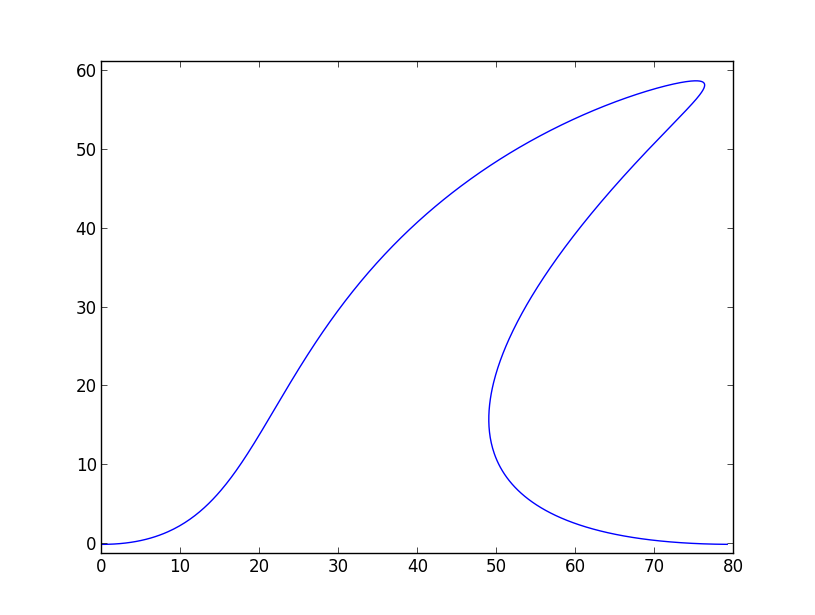
\includegraphics[width=.9\textwidth]{images/shark.png}
\textit{Tracé d'une courbe de Bézier}
\end{center}
\end{minipage}

\vspace{.5cm}


%\begin{center}
%\includegraphics[width=.9\textwidth]{png/cyclev.png}

%\textit{Cycle de conception d'un produit}
%\end{center}

%\begin{prob}
%\textsc{Problématique :}

%En phase d'avant conception d'un produit, quels sont les critères qui vont permettre de choisir les matériaux à utiliser ?
%\end{prob}

Le tracé de ces courbes fait appel à la définition de fonctions, de boucles, d'instructions conditionnelles qui sont au c\oe{}ur du développement de programmes informatiques. 

Le but de ce cours est de définir les instructions de base qui doivent permettre la réalisation d'algorithmes. 

\begin{savoir}
\textsc{Savoirs :}
\begin{itemize}
\item Instructions conditionnelles
\item Instructions itératives
\item Fonctions
\end{itemize}
\end{savoir}
 

\setlength{\parskip}{0ex plus 0.2ex minus 0ex}
 \renewcommand{\contentsname}{}
 \renewcommand{\baselinestretch}{1}

\tableofcontents

 \renewcommand{\baselinestretch}{1.2}
\setlength{\parskip}{2ex plus 0.5ex minus 0.2ex}

% \vspace{1cm}
\textit{Ce document évolue. Merci de signaler toutes erreurs ou coquilles.}


\section{Syntaxe}

\subsection{Sémantique}
\begin{defi}
Lors de l'exécution d'un programme, les instructions s'exécutent les unes après les autres dans leur ordre d'écriture.

Une séquence d'instructions s'appelle un bloc d'instruction.
\end{defi}



\begin{exemple}
%\begin{minipage}[c]{.3\linewidth}

\begin{pseudo}
\begin{algorithm}[H]
Instruction 1
\Fonction{
Instruction 1\\
...\\
Instruction 2\\
}
\end{algorithm}
\end{pseudo}
%\end{minipage}\hfill
%\begin{minipage}[c]{.3\linewidth}
En python, les instructions peuvent être séparées par des retours à la ligne, des points-virgules. Dans le cas des blocs d'instructions, les instructions sont indentées (4 espaces). 
\begin{py}
\begin{minipage}{.9\linewidth}
\begin{python}[showspaces=true]
Instruction1
Instruction2
Instruction1;Instruction2
Bloc : 
    Instruction 1
    Instruction 2
\end{python}
\end{minipage}
\end{py}
%\end{minipage}\hfill
%\begin{minipage}[c]{.3\linewidth}
En Scilab : une virgule, un point virgule, un retour à la ligne peuvent séparer des instructions. (Lorsque les instructions sont terminées par un point virgule, les résultats des instructions ne sont pas affichées à l'écran.)

Les blocs sont terminés par \textsf{end}.
\begin{sci}
\begin{scilab}
Instruction1
Instruction2
Instruction1,Instruction2
Instruction1;Instruction2;
Debut Bloc
Instruction 1
Instruction 2
end
\end{scilab}
\end{sci}
\end{exemple}


\subsection{Définition de fonctions}
\subsubsection{Les fonctions}
Lors de l'exécution d'un programme, il est très courant qu'une même séquence d'instruction soit répété un grand nombre de fois. Ainsi, il est courant de décomposer un problème sous forme de plusieurs sous programmes élémentaires. 

%\begin{defi}

%\end{defi}


\begin{exemple}
\textit{Courbes de Bézier d'ordre 2}

Prenons le cas où nous souhaitons connaître les coordonnées d'un point appartenant à une courbe de Bézier définie par 3 points. 
Dans ce cas,
$$
\forall u \in [0,1] \quad 
\left\{
\begin{array}{l}
x(u)= \left(1-u\right)^2 x_0 + 2u\left(1-u\right)x_1 + u^2 x_2\\
y(u)= \left(1-u\right)^2 y_0 + 2u\left(1-u\right)y_1 + u^2 y_2
\end{array}
\right.
$$

Écrivons la fonction permettant d'évaluer une coordonnée en un paramètre donné. Autrement dit :
$$
\forall u \in[0,1] f(u)= \left(1-u\right)^2 x_0 + 2u\left(1-u\right)x_1 + u^2 x_2
$$


\begin{pseudo}
\begin{algorithm}[H]
\Donnees{u,$x_0$,$x_1$,$x_2$}

\Fonction{
Fonction $f(u,x_0,x_1,x_2)$:\\
$val \gets (1-u)^2x_0 + 2u(1-u)x_1 + u^2x_2$\\
\Retour{val}
}
print $f(0.5,0,1,2)$  
\end{algorithm}
\end{pseudo}

\begin{py}
\begin{python}
def f(u,x0,x1,x2):
    val = (1-u)**2*x0 + 2*u*(1-u)*x1 + u**2*x2
    return val

print(f(0.5,0,1,2))    
\end{python}
\end{py}

\begin{sci}
\begin{scilab}
function [val]=f(u,x0,x1,x2)
  val=(1-u)**2*x0+2*u*(1-u)*x1+u**2*x2;
endfunction

printf("%f",f(0.5,0,1,2))
\end{scilab}
\end{sci}

Dans ce cas, rien ne permet de contrôler que $u$ appartient bien à l'intervalle 
$[0,1]$ et que les arguments $x0$, $x1$, et $x2$, sont bien des nombres réels.
\end{exemple}

\subsubsection{Variables locales -- Variables globales}

\begin{defi}
\textbf{Visibilité :}

Une variable globale est définie en dehors de toute fonction, une variable locale est définie dans une fonction et masque toute autre variable portant le même nom.

\textbf{Durée de vie :}

Une variable globale existe durant l'exécution du programme, une variable locale existe durant l'exécution de la fonction.

\textbf{Par défaut, dans un langage interprété, les variables sont locales à un bloc.}
\end{defi}



\begin{exemple}
\textit{Courbes de Bézier d'ordre 2}

On reprend le cas précédent. On se place dans le cas où le programme n'utilise que des courbes Bézier d'ordre 2 et où les pôles restent inchangés. On souhaite alors définir la fonction $f$ sans avoir à rappeler les coordonnées de chacun des pôles.

 

\begin{pseudo}
\begin{algorithm}[H]
\Donnees{u}
\Donnees{Global : $x_0\gets 0$,$x_1\gets 1$,$x_2\gets 2$}
\Fonction{
Fonction $f(u)$:\\
$val \gets (1-u)^2x_0 + 2u(1-u)x_1 + u^2x_2$\\
\Retour{val}
}
print $f(0.5)$
\end{algorithm}
\end{pseudo}
\begin{py}
\begin{python}
def fx(u):
    val = (1-u)**2*x0 + 2*u*(1-u)*x1 + u**2*x2
    return val
    
global x0,x1,x2
x0,x1,x2=0,1,2

print(fx(0.5))  
\end{python}
\end{py}

\begin{sci}
\begin{scilab}
function [val]=f(u)
  val=(1-u)**2*x0+2*u*(1-u)*x1+u**2*x2;
endfunction

global x0 x1 x2
x0=0;x1=1;x2=2;

printf("%f",f(0.5))
\end{scilab}
\end{sci}

\end{exemple}

\begin{rem}
De manière générale, on essaiera d'utiliser le moins possible les variables globales.
\end{rem}

%\subsubsection{Attributs d'un objet}

%Visibilité des attributs d'un objet : publique, protégée et privée selon la définition de l'objet.

\subsubsection{Documentation des fonctions}
En programmation, il est indispensable de documenter les fonctions. En effet, il n'est pas toujours facile de se replonger dans un algorithme qu'on a écrit et il est indispensable de le ponctuer de commentaires pour pouvoir bien comprendre le but d'une fonction, d'une boucle \textit{etc}.

\begin{py}
En python un commentaire court commence par le signe \#. 

Les commentaires longs sont encadrés par trois guillemets ".

\begin{python}
# ======= Debut de la definition des fonctions =======
def f(u,x0,x1,x2):
    """
    Retourne la coordonnee d'un point pour une courbe de Bezier d'ordre 2
    Keyword arguments:
    u -- parametre de la courbe parametree (doit etre compris entre 0 et 1)
    x0 -- coordonnee du pole 0 (sur x, y ou z)
    x1 -- coordonnee du pole 1 (sur x, y ou z)
    x2 -- coordonnee du pole 2 (sur x, y ou z)
    """
    val = (1-u)**2*x0 + 2*u*(1-u)*x1 + u**2*x2
    return val
# ======= Fin de la definition des fonctions =======
\end{python}

Lorsqu'une fonction est commentée comme dans l'exemple ci-dessus, on peut accéder à de la documentation sur la fonction en procédant ainsi :
\begin{python}
>>> help(f)
>>> f.__doc__
\end{python}

Enfin, sous linux, il est possible de générer automatiquement de la documentation au format \textsf{html} :

\textsf{pydoc -w ./ExempleCours.py} 
\end{py}

\begin{sci}

En scilab un commentaire commence par un double slash : //. 

\begin{scilab}
// La fonction f etourne la coordonnee d'un point pour une courbe de Bezier d'ordre 2
//     * u : parametre 
//     * x0, x1, x2 coordonnees des poles 0 1 et 2
function [val]=f(u,x0,x1,x2)
  val=(1-u)**2*x0+2*u*(1-u)*x1+u**2*x2;
endfunction
\end{scilab}
\end{sci}

\subsection{Import de fonctions}

Par défaut, Python ne permet que de réaliser des opérations élémentaires (opérations mathématiques élémentaires, comparaisons, boucles \textit{etc.}). 

Il existe par ailleurs un grand nombre de bibliothèques permettant par exemple de manipuler des fonctions mathématiques ($\sin$, $\cos$, $\sqrt{\;}$ \textit{etc.}), des bibliothèques permettant de tracer des courbes, des bibliothèques permettant d'interroger des bases de données \textit{etc.}

 

\begin{exemple}
Pour utiliser les méthodes liées à ces bibliothèques, on procèdera ainsi :

\begin{py}
\begin{python}
import math  # Import de toutes les methodes de la bibliotheque math
math.sqrt(2) # Permet d'utiliser la methode sqrt de la bibliotheque math
from math import sqrt # Import de la methode sqrt de la bibliotheque math

import os # Import de la bibliotheque os permettant de realiser des operations systemes
\end{python}
\end{py} 
\end{exemple}

\begin{warn}
Il est déconseillé d'utiliser la méthode d'import suivante : 
\begin{python}
from os import *
\end{python}

En effet, si des méthodes ont le même nom, seules les méthodes de la dernière bibliothèque sont utilisables. 
\end{warn}



\section{Instructions conditionnelles}



\subsection{Expressions booléennes}
\begin{defi}
Une expression booléenne est une instruction qui renvoie la valeur "vrai" ou "faux".
\end{defi}

\begin{defi}
\textbf{Opérateurs de comparaison}


\begin{minipage}[c]{.3\linewidth}

\begin{pseudo}
\begin{algorithm}[H]
$2=8 $ \\
$2\neq8 $\\
$2\geq 8 $\\
$2>8 $\\
$2\leq 8$\\
$2<8$\\
\end{algorithm}
\end{pseudo}

\end{minipage} \hfill
\begin{minipage}[c]{.3\linewidth}
\begin{py}
\begin{python}
 >>> 2==8
	False
 >>> 2!=8
	True
 >>> 2>=8
	False
 >>> 2>8
	False
 >>> 2<=8
	True
 >>> 2<8
	True
\end{python}
\end{py}
\end{minipage} \hfill
\begin{minipage}[c]{.3\linewidth}
\begin{sci}
\begin{scilab}
 --> 2==8
	F
 --> 2!=8
	T
 --> 2>=8
	F
 --> 2>8
	F
 --> 2<=8
	T
 --> 2<8
	T
\end{scilab}
\end{sci}
\end{minipage}

\end{defi}


\begin{exemple}

\end{exemple}


\subsection{Boucle \textsl{Tant que}}

\begin{defi}
La boucle \textsf{Tant que} appelée aussi boucle \textsf{while} permet de répéter une instruction tant qu'une condition reste vraie.
\end{defi}

\begin{rem}
Les boucles ont la plupart du temps besoin d'être incrémentées. Pour cela plusieurs solutions sont possibles.

\begin{minipage}[c]{.3\linewidth}
\begin{pseudo}
\begin{algorithm}[H]
$i \gets 1$\\
$i \gets i+1$\\
\end{algorithm}
\end{pseudo}
\end{minipage} \hfill
\begin{minipage}[c]{.3\linewidth}
\begin{py}
\begin{python}
>>> i=1
>>> i=i+1;print(i)
    2
>>> i+=1;print(i)
    3
>>> i+=2;print(i)
    5
\end{python}
\end{py}
\end{minipage} \hfill
\begin{minipage}[c]{.3\linewidth}
\begin{sci}
\begin{scilab}
--> i=1;
--> i=i+1;
\end{scilab}
\end{sci}
\end{minipage} 

\end{rem}


\begin{exemple}
\textit{Implémentation de la fonction "factorielle"}

On peut définir la fonction factorielle ainsi : 
$$
\forall  n\in \mathbb{N}
\left\{
\begin{array}{l}
\text{si } n=0 \quad n!=1\\
\text{sinon } n !=\prod\limits_{i=1}^n i
\end{array}
\right.
$$
 
On s'intéresse à la programmation du cas où $n$ est supérieur ou égal à 1.

\begin{minipage}[c]{.3\linewidth}
\begin{pseudo}
\begin{algorithm}[H]
\Fonction{
factorielle($n$):\\
$i\gets1$\\
$res\gets1$\\
\Tq{$i\leq n$}{
$res \gets res \cdot i$ \\
$i\gets i+1$}
\Retour{res}
}
\end{algorithm}
\end{pseudo}
\end{minipage}\hfill
\begin{minipage}[c]{.3\linewidth}
\begin{py}
\begin{python}
def factorielle(n):
        i=1    
        res=1
        while i<=n:
            res=res*i
            i+=1
        return res
\end{python}
\end{py}
\end{minipage}\hfill
\begin{minipage}[c]{.3\linewidth}
\begin{sci}
\begin{scilab}
function [res]=factorielle(n)
  i=1;
  res=1;
  while i<=n
    res = res*i
    i=i+1
  end
endfunction
\end{scilab}
\end{sci}
\end{minipage}

\end{exemple}



\begin{warn}
Lors de la réalisation d'une boucle \textsl{while} il faut veiller à ce que l'instruction conditionnelle change d'état afin de sortir de la boucle et de ne pas provoquer une boucle sans fin...
\end{warn}


\subsection{Instruction \textsl{Si, Sinon}}

\begin{defi}
La boucle \textsf{Si} appelée aussi boucle \textsf{if} permet d'exécuter une instruction si une condition est vraie.
\end{defi}


\begin{exemple}
\textit{Implémentation de la fonction "factorielle"}

On souhaite maintenant gérer le cas où $n=0$. Dans ce cas, le calcul de $!n$ est différent du cas où $n>0$.

\begin{minipage}[c]{.35\linewidth}
\begin{pseudo}
\begin{algorithm}[H]
\Fonction{
factorielle($n$):\\
\eSi{n=0}{
\Retour{1}
}{
$i\gets1$\\
$res\gets1$\\
\Tq{$i\leq n$}{
$res \gets res \cdot i$ \\
$i\gets i+1$}
\Retour{res}
}}
\end{algorithm}
\end{pseudo}
\end{minipage}\hfill
\begin{minipage}[c]{.3\linewidth}
\begin{py}
\begin{python}
def factorielle(n):
    if n==0:
        return 1
    else :
        i=1    
        res=1
        while i<=n:
            res=res*i
            i+=1
        return res
\end{python}
\end{py}
\end{minipage}\hfill
\begin{minipage}[c]{.3\linewidth}
\begin{sci}
\begin{scilab}
function [res]=factorielle(n)
  if n==0
    res =1;
  else
    i=1;
    res=1;
    while i<=n
      res = res*i
      i=i+1
    end
  end  
endfunction
\end{scilab}
\end{sci}
\end{minipage}

\textit{Remarque :} Il faudrait vérifier que $n$ est bien un \textbf{entier} \textbf{positif ou nul}.
\end{exemple}


\begin{exemple}
\textit{Implémentation de la fonction "factorielle"}

On souhaite maintenant s'assurer que $n$ est bien un \textbf{entier} \textbf{positif ou nul}.


%\begin{pseudo}
%En pseudo-code
%\end{pseudo}

\begin{py}
\begin{python}
def calc_factorielle(n):
    if (type(n)==int) & (n>=0):
        return factorielle(n) 
    else :
        print("Oooops... il faut saisir un nombre entier POSITIF ou nul")
\end{python}
\end{py}

%\begin{sci}
%\begin{scilab}
%Scilab
%\end{scilab}
%\end{sci}

\textit{Remarque :} Il faudrait vérifier que $n$ est du bon type.
\end{exemple}


\subsubsection*{La gestion des erreurs}


\begin{exemple}
\textit{Implémentation de la fonction "factorielle"}

On souhaite maintenant s'assurer que $n$ est du bon type.

%\begin{pseudo}
%E pseudo-code
%\end{pseudo}

\begin{py}
\begin{python}[moreemph={[4], 46, 48}]
def calc_factorielle(n):
    try:
        if (type(n)==int) & (n>=0):
            return(factorielle(n))
        else :
            print("Oooops... il faut saisir un nombre entier POSITIF ou nul")
    except TypeError:
        print("Oooops... le type de la variable n'est pas le bon")
\end{python}
\end{py}

%\begin{sci}
%\begin{scilab}
%Scilab
%\end{scilab}
%\end{sci}

\end{exemple}


\begin{rem}
Pour aller plus loin : on peut définir ses propres exceptions et gérer les messages d'erreur. 
\begin{py}
\begin{python}
class MonException(Exception):
    def __init__(self,raison):
        self.raison = raison
     
    def __str__(self):
        return self.raison
 
def calc_factorielle(n):
    if n > 20:
        raise MonException("Il faut saisir un entier positif ou nul")
    else:
        return factorielle(n)
\end{python}
\end{py}
\end{rem}



%\begin{itemize}
%\item Expressions booléennes et opérateurs logiques simples.
%\item Sémantique (fond)
%\item Syntaxe (forme) : instructions 	
%\begin{itemize}
%\item si, sinon (pseudo langage)
%\item if, elif, else (python)
%\item if, then, else, elseif, select, case, end (scilab)
%\end{itemize}
%\item Problème d’une comparaison avec un nombre réel. Le type float est le plus souvent une %approximation
%\end{itemize}



\section{Instructions itératives}

\begin{defi}
Une instruction itérative permet de répéter une suite d'instructions un nombre déterminé de fois. 
On parle aussi de boucle \textsf{for}.
\end{defi}

%\begin{rem}
%Incréments range...
%\end{rem}

\begin{exemple}
\textit{Courbes de Bézier d'ordre 2}

Nous avons précédemment étudié la fonction permettant de calculer l'abscisse ou l'ordonnée d'un point d'une courbe de Bézier. 

Pour afficher une telle courbe une solution consiste en calculer les coordonnées d'un nombre $n$ de points et de relier ces points par des segments de droite. Plus le nombre de points sera élevé plus la courbe paraîtra lisse, mais le temps de calcul sera d'autant plus élevé. On rappelle qu'une courbe de Bézier est une courbe paramétrique définie pour $u\in[0;1]$ et que la fonction $f$ est définie par $f(u)=\left(1-u\right)^2x_0 + 2u\left(1-u\right)x_1+u^2x_2$.

Il va falloir \textbf{discrétiser} l'intervalle $[1,0]$.
\end{exemple}

\newpage

\begin{exemple}
\begin{minipage}[c]{.36\linewidth}
\begin{pseudo}
\begin{algorithm}[H]
Tableau $x$;\\
Tableau $y$;\\
$x_0 \gets 0$; $y_0 \gets 0$\\
$x_1 \gets 10$; $y_1 \gets 10$\\
$x_2 \gets 20$; $y_2 \gets 0$\\
$i \gets 0$; $n \gets 50$\\
\Pour{i de 0 à $n$}{
$u \gets i/(n-1)$\\
$ x[i] \gets f(u,x_0,x_1,x_2)$\\
$ y[i] \gets f(u,y_0,y_1,y_2)$\\
$i \gets i+1$\\
}
Afficher($x$,$y$)
\end{algorithm}
\end{pseudo}
\end{minipage}\hfill
\begin{minipage}[c]{.3\linewidth}
\begin{py}
\begin{python}
import numpy as np
import pylab as pl

x0=0;y0=0
x1=10;y1=10
x2=20;y2=0
n=50
x,y=[],[]
for i in range(0,n):
    u=i/(n-1)
    x.append(f(u,x0,x1,x2))
    y.append(f(u,y0,y1,y2))
pl.plot(x,y)
pl.axis('equal')
pl.show()
\end{python}
\end{py}
\end{minipage}\hfill
\begin{minipage}[c]{.3\linewidth}
\begin{sci}
\begin{scilab}
x0=0;y0=0;
x1=10;y1=10;
x2=20;y2=0;
n=50;
for i=1:n
  u=i/n;
  x(i)=f(u,x0,x1,x2);
  y(i)=f(u,y0,y1,y2);
end
plot2d(x,y) // a verifier
\end{scilab}
\end{sci}
\end{minipage}



\begin{minipage}[c]{.22\linewidth}
\begin{center}
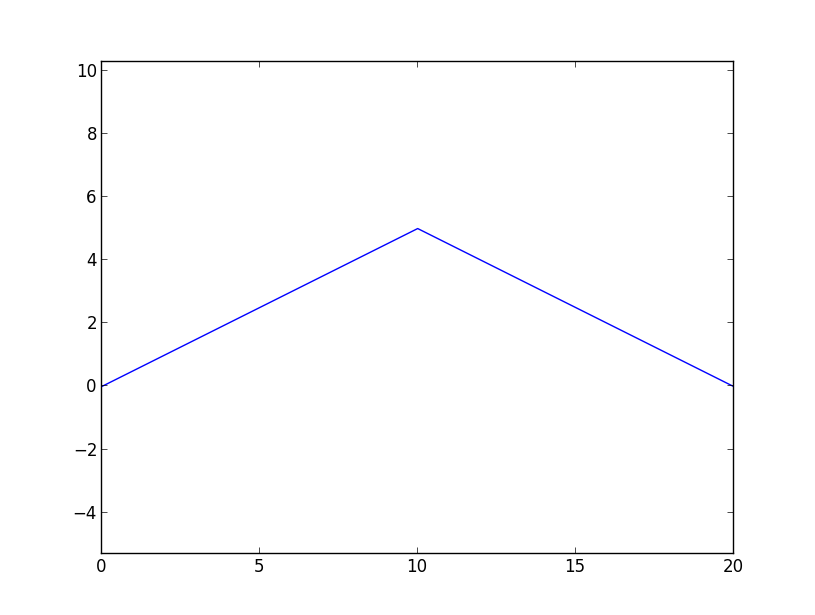
\includegraphics[width=\textwidth]{images/n3}

$n=3$
\end{center}
\end{minipage}\hfill
\begin{minipage}[c]{.22\linewidth}
\begin{center}
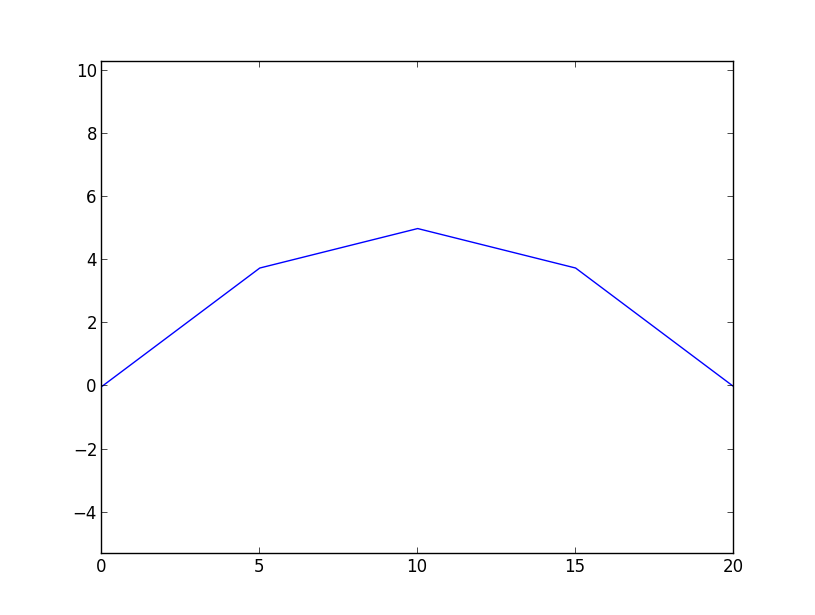
\includegraphics[width=\textwidth]{images/n5}

$n=5$
\end{center}
\end{minipage}\hfill
\begin{minipage}[c]{.22\linewidth}
\begin{center}
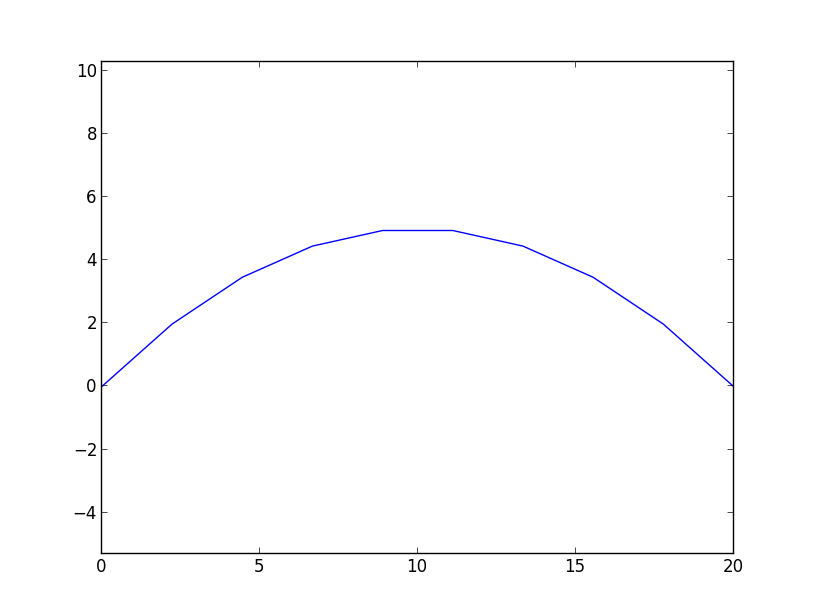
\includegraphics[width=\textwidth]{images/n10}

$n=10$
\end{center}
\end{minipage}\hfill
\begin{minipage}[c]{.22\linewidth}
\begin{center}
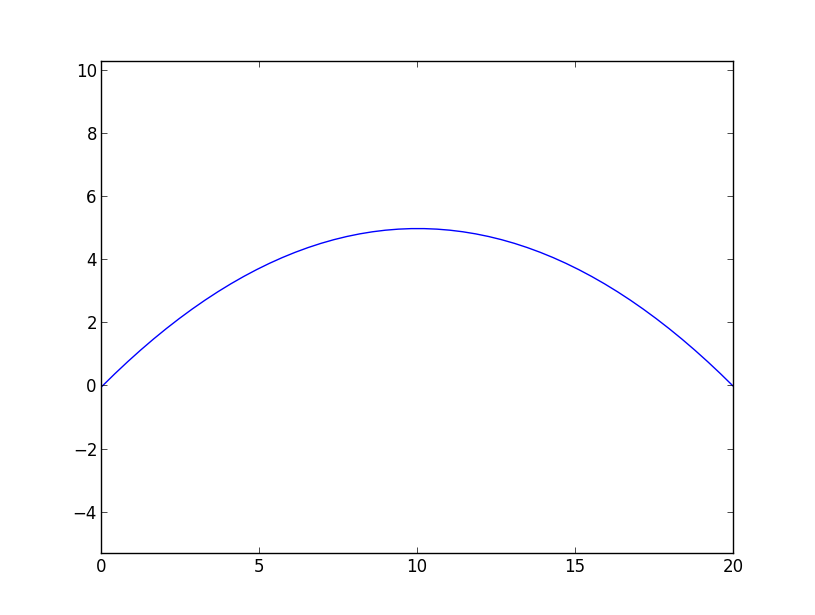
\includegraphics[width=\textwidth]{images/n50}

$n=50$
\end{center}
\end{minipage}
\end{exemple}


\begin{rem}
En python, \textsf{range} permet de définir la liste des valeurs qui vont être utilisées lors du parcours de la boucle \textsf{for}.  Cette fonction peut prendre jusqu'à 3 arguments : le premier argument désigne la valeur de départ, le second la valeur de fin (exclue), la troisième la valeur de l'incrément. 
\end{rem}

\begin{rem}
La boucle \textsf{while} définie précédemment est aussi une instruction itérative. 
\end{rem}


\begin{exemple}
\textit{Courbes de Bézier d'ordre 2}


%\begin{pseudo}
%En pseudo-code
%\end{pseudo}

\begin{py}
\begin{python}
inc = 0.1
while u<=1 :
    x.append(f(u,x0,x1,x2))
    y.append(f(u,y0,y1,y2))
    u += inc
\end{python}
\end{py}

\begin{sci}
\begin{scilab}
inc = 0.1; i = 1;
u=0;
x = []; y = [];
while u<=1
    x(i)=f(u,x0,x1,x2);
    y(i)=f(u,y0,y1,y2);
    u=u+inc;
    i=i+1;
end
\end{scilab}
\end{sci}

\end{exemple}




%\section{Création de fonctions}

%\subsection{Définition}

%\subsection{Portée des variables}

%Fonctions et procédures
%
%Nécessité de décomposer un problème an sous-problèmes élémentaires.
%Fonctions
%-	notion de fonction (au sens informatique),
%-	définition dans le langage utilisé :
%pseudo langage : type de retour fonction (types et arguments) { …. retourner valeur }
%python : def, return 
%scilab : function, endfunction
%-	paramètres (ou arguments)
%Une fonction a une liste de paramètres types.
%Le passage de paramètres se fait par valeur pour les types simples.
%Quand le type du paramètre est composite, les éléments du tableau ou les champs des structures sont par contre modifiés par le code de la fonction.
%Valeurs par défaut
%Arguments avec étiquettes
%-	résultats
%Une fonction a un type de retour (son prototype ou sa signature)




%python
%def produit_scalaire(u,v):
%	r=0
%	for i in range(1,3):
%		r=r+u[i]*v[i]
%	return r
%x=produit_scalaire([1,2,3],[0,1,2])	scilab
%function [r]=produidef f(u):
% ????
%r=0
%for i=1:3, r=r+u(i)*v(i), end
%endfunction
%
%x=produit_scalaire([1,2,3],[0,1,2])
%Les fonctions doivent être largement documentées.
%Modules de fonctions
%Ensemble de fonctions regroupées dans un fichier
%Python : from module import *, import module, from math import sqrt
%
%Fonctions et méthodes
%Sensibilisation aux méthodes associées aux objets (python est naturellement orienté objet).
%Cela sera largement utile dans l’utilisation de bibliothèques d’interfaces graphiques, dans la manipulation des fichiers. 
%Le champ d’un objet peut être un attribut qui fait partie de sa structure (ex : eleve.nom=Dupont) ou une méthode (ex : eleve.ajouter(Dupont, Pierre)).
%
%Exemple :
%>>> t=["2"]
%>>> t.append("4") 	#« append » est une méthode (fonction) utilisable sur un objet de type liste.
%>>> t
%['2', '4']
%>>> type (t)
%<class 'list'> 

\end{document}





\end{document}
